\documentclass[12pt, a4paper]{article}
\PassOptionsToPackage{sharp}{prettytex/boxes}
\usepackage{prettytex/base}

\setlength{\topmargin}{0.0in}
\setlength{\oddsidemargin}{0.33in}
\setlength{\textheight}{9.0in}
\setlength{\textwidth}{6.0in}
\renewcommand{\baselinestretch}{1.25}

\usepackage{prettytex/math}
\usepackage[nameinlink]{cleveref}
\usepackage[cleveref]{prettytex/math-theorems}
\usepackage{prettytex/mathematicians}
% \usepackage{prettytex/gfx}
% \usepackage{prettytex/code}
\usepackage{prettytex/pseudo}
\usepackage{prettytex/thesis}
\usepackage{tabularray}
\usepackage{cancel}
\usepackage{bbm}

\setlength{\headheight}{19.53pt}
\setlength{\headsep}{1.8em}
\addbibresource{sources.bib}
\AfterEndEnvironment{minted}{\vspace*{-0.8cm}}
\renewcommand{\operatorcolor}{black}

\newcommand{\identity}{\mathbbm{1}}
\let\oldemptyset\emptyset
\let\emptyset\varnothing

\newcommand{\topictitle}{Unsupervised Semantic Field Analysis \\ \large using Community Detection Methods}
\newcommand{\candidatenumber}{1072462}
\newcommand{\course}{Networks}

\title{\topictitle}
\author{Candidate \candidatenumber}
\date{\today}

% ✅ Prepare report
% ✅ Insert a few pictures from references maybe
% ✅ in the introduction, mention all the methods described by Fortunato et al. (lots of text)
% ✅ derive the modularity gain described in the Louvain paper
% ✅ use / plot https://www.mapequation.org/infomap/
% ✅ analyze the Eigengap which tells the amount of clusters
% Try out Simulated Annealing? (Fortunato) -- works really well (cf. Fortunato Table 1)
% analyze / mention: is the network small-world or not?
% maybe cite Lambiotte's book

\begin{document}
  \pagestyle{plain}
  \begin{center}
    \vspace*{-2.5cm}
    \Large \topictitle \\
    \vspace{.3cm}

    \normalsize Special Topic on \textcolor{themecolor3}{\textsc{\course}}\\
    \normalsize Candidate Number: \textcolor{themecolor3}{\candidatenumber}
    \vspace{.3cm}
  \end{center}

  \begin{abstract}
    \label{abstract}
    In this work we will attempt to compare methods in the domain of semantic field tagging by considering a language literature corpus as a large graph of neighbouring words. The network is built by performing part-of-speech tagging iteratively on the entire corpus and linking together principal words that are connected in a neighbouring sense up to a radius of $r$ words.
    The resulting graph $G_r$ is then analysed using community detection methods such as \textit{Louvain Clustering}, \textit{Chinese Whispers}, \textit{Clauset Greedy Modularity} and other clustering approaches which we only discuss briefly.
    We derive the gain in modularity presented in the original work \cite{lambiotte-louvain-clustering} upon atomic modification of the clusters $\{C_i\}_{i=1}^{n_C}$.
    The Chinese Whispers algorithm is a simple graph clustering method originating from research in Natural Language Processing \parencite{cw-biemann} and it is well-established for semantic field analysis.
    The abovementioned algorithms are applied to a real-world corpus of the Latin language, working with a graph of 10843 nodes and 2.4 million edges.
    We compare them in terms of output modularity, runtime and number of clusters on the graphs introduced, which we compare to the eigengap in the spectrum of the graph Laplacian.
  \end{abstract}

  \begin{figure}[H]
    \centering
    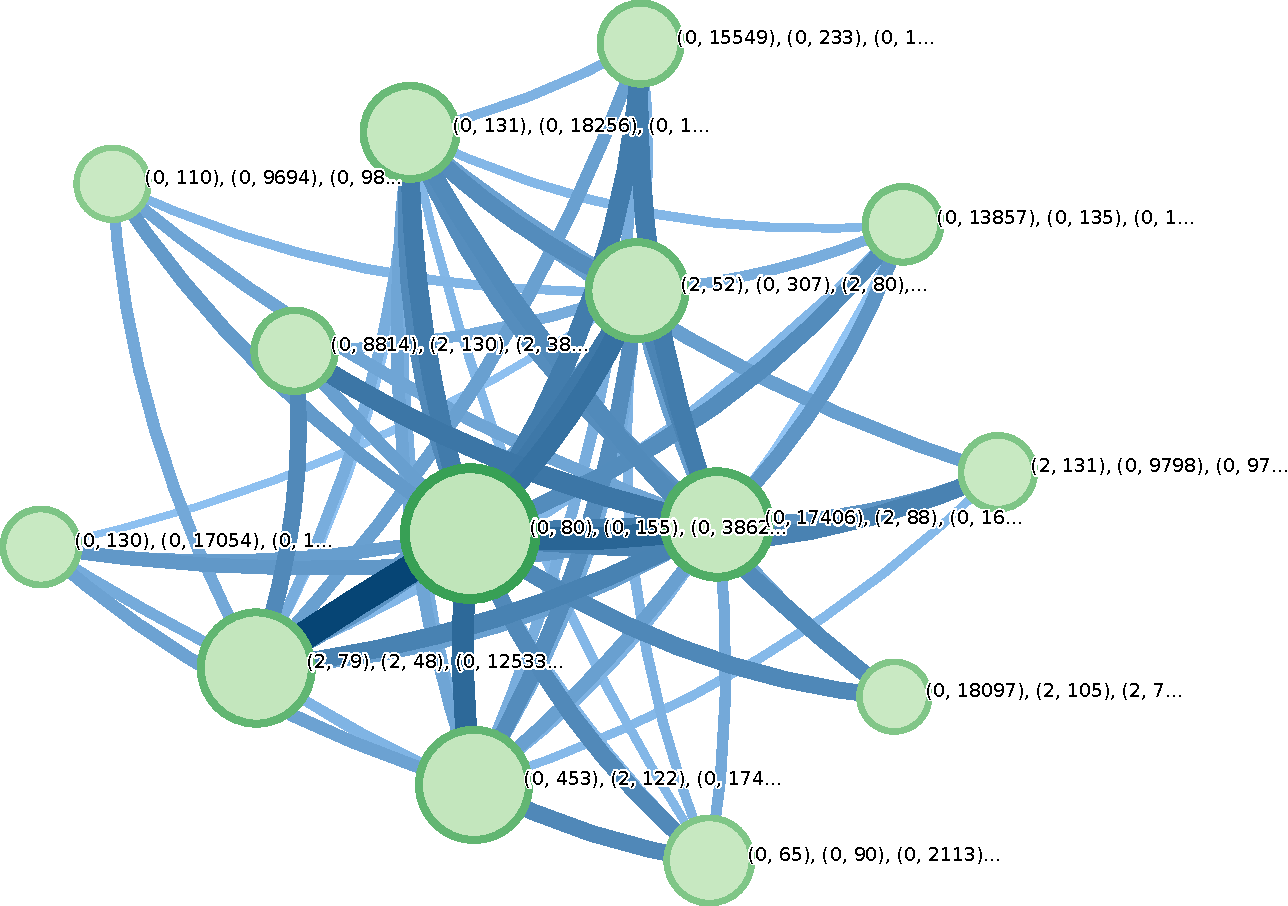
\includegraphics[width=0.65\linewidth]{figures/library-graph-12.pajek.ftree.pdf}
    \caption{Visualisations of a clustering of the corpus generated semantic network $G_{12}$, obtained using the Map Equation approach (cf. \Cref{sec:mapequation}). Visualised using the InfoMap visualisation package \parencite{mapequation}, where the labels indicate database references.}
    \label{fig:mapequation}
  \end{figure}

  \pagebreak
  \pagestyle{normal}

  \tableofcontents
  \pagebreak

  \section{Introduction}
  Let $\N = \Z^+$ denote the positive integers and $N_0 := \{0\} \cup \N$ the nonnegative integers.

  The methods we will discuss to identify semantic fields will be based on graph clustering algorithms applied to a text corpus word connectedness / neighbourhood network $G_r$.
  As we will discuss later, different neighbourhood radii $r \in \N$ give us different insight into the structure of a natural language.
  We will focus our attention on methods for undirected graphs, ``graphs without direction'' (cf. \Cref{def:undirected-graph}) and without loops.
  \begin{definition}{Undirected Graph}{undirected-graph}
    A graph $G = (V, E)$ with vertices $V$ and edges $E \subseteq V \times V$ is undirected if and only if $(v_i, v_j) \in E \Rightarrow (v_j, v_i) \in E \quad \forall\; v_i, v_j \in V$.
  \end{definition}

  Vertices are also referred to as \textit{nodes}.
  Every graph $G$ is uniquely described by its adjacency matrix $A \in \{0, 1\}^{n \times n}$ (\Cref{def:adjacency-matrix}), which allows us to talk about ``linear algebra'' of graphs, which is especially relevant to spectral graph clustering methods (cf. \Cref{sec:spectral-clustering}).

  \begin{definition}{Adjacency Matrix}{adjacency-matrix}
    Let $A \in \{0, 1\}^{n \times n}$ denote the symmetric adjacency matrix of an undirected graph $G = (V, E)$. Its entries are given by $a_{ij} = \{A\}_{ij} = \identity_{(v_i, v_j) \in E}$, so $a_{ij} = 1$ if vertex $v_i$ is connected to $v_j$ and $0$ otherwise.
  \end{definition}

  By construction, $A = A^T$ is symmetric and has all-$0$s in the diagonal (no loops), a definition that corresponds to the fact that you cannot be friends with yourself in a social network.

  Further let $m := |E|$ and $n := |V|$ denote the number of edges and vertices, respectively.
  The degree $d_i$ of a vertex $v_i \in V$ is defined by the number of edges connecting to it, so $$d_i := \deg(v_i) = \big|\left\{(v_j, v_k) \in E \;|\; v_j = v_i\right\}\big|\,,$$ for an undirected graph $G = (V, E)$. The handshaking lemma (\Cref{lemma:handshaking}) tells us an important fact useful for normalisation.
  \begin{lemma}{Handshake}{handshaking}
    For every finite, undirected graph $G = (V, E)$ the individual vertex degrees sum up to exactly twice the number of edges, so $$\sum_{i=1}^{n} d_i = \sum_{v \in V} \deg(v) = 2m\,.$$
  \end{lemma}

  The individual vertex degrees can be summarised in the so-called \textit{degree matrix} $D := \diag(d_1, ..., d_n)$, $D \in \N_0^{n \times n}$. The graph \textit{Laplacian} is defined by $L := D - A$.

  Given a graph, we are interested in performing \textbf{graph clustering}, also referred to as \textbf{community detection} or \textbf{graph partitioning}, the goal of which is to obtain a set of mutually exclusive clusters $C_i \subseteq V$ (cf. \Cref{def:clustering}).
  The term \textit{graph partitioning} is more frequently used in the context of minimal cuts, where one aims to minimise each \textit{cut size} referring to the number of edges in between clusters.

  Note that in the scope of this report we only consider an unweighted, undirected graph, while most clustering algorithms also allow working with a weighted graph $\tilde{G} = (V, \tilde{E})$ where $\tilde{E} \subset V \times V \times \R^+$ is a set of three-tuples $(v_i, v_j, w_{ij})$ instead of vertex pairs. Or equivalently, one can define a function $w: \tilde{E} \mapsto \R^+$ which maps vertex pairs (edges) to their respective weight.

  \begin{definition}{Graph Clustering}{clustering}
    Let $C = \left\{C_i \subseteq V \right\}_{i=1 ... n_C}$ denote a clustering of $G = (V, E)$ into $n_C \in \N$ clusters where $C_i \cap C_j = \emptyset \; \forall\,i, j \in \{1, ..., n_C\}$ and $\bigcup_{i=1}^{n_C} C_i = V$. Let $s_i \in \{1, ..., n_C\}$ denote the assigned cluster of vertex $v_i \in V$.
  \end{definition}

  \begin{figure}[h]
    \centering
    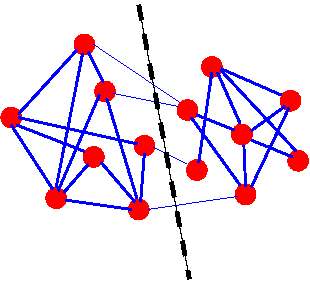
\includegraphics[width=0.3\linewidth]{figures/graphpartitioning.pdf}
    \caption{Partitioning of a graph using \textit{cuts} \parencite{fortunato-2009}.}
  \end{figure}

  These clusterings may be better or worse depending on the context, but a generally solid measure of ``clustering goodness'' is \textit{modularity} (\Cref{def:modularity}).

  \begin{definition}{Modularity}{modularity}
    For a given undirected graph $G = (V, E)$ and clustering $C$, let $$Q := \frac{1}{2m} \sum_{i=1}^{n} \sum_{j=1}^{n} \left(A_{ij} - \frac{d_i d_j}{2m}\right) \delta(s_i, s_j)\,,$$ with $\delta(\cdot, \cdot)$ the Kronecker delta indicating whether two vertices $v_i$ and $v_j$ belong to the same cluster \parencite{lambiotte-louvain-clustering}.
  \end{definition}

  Modularity is a measure of the quality of a clustering (also referred to as a partitioning) of $G$. It can also be written as the sum of individual cluster contributions
  $$Q = \sum_{c=1}^{n_C} Q_c = \frac{1}{2m} \sum_{c=1}^{n_C} \left[\sum_{v_i \in C_c} \sum_{v_j \in C_c} \left(A_{ij} - \frac{d_i d_j}{2m}\right)\right]\,,$$
  which might make its purpose a bit clearer.

  \begin{figure}[H]
    \centering
    \includegraphics[width=0.56\linewidth]{figures/nice-modularity.eps}
    \caption{Four clustered graphs along with their modularity $Q$ (and map equation value $L$, cf. \cite{mapequation} and \Cref{sec:mapequation}) to provide a visual illustration of modularity. Source: \cite{mapequation}.}
  \end{figure}

  \section{Clustering Methods and Algorithms}
  In the context of Natural Language Processing, graph clustering methods can be employed for various tasks such as word sense induction or language separation.
  In this work however, we will only focus on semantic field tagging.

  Most clustering methods can be broadly categorised into spectral, partitional (such as k-means clustering), hierarchical, randomised, divisive and quality-optimisation algorithms \parencite{fortunato}.
  % An interesting approach is Markov-Chain-Clustering, which may employ Simulated Annealing.

  Community detection is, in principle, usually a ``very hard'' task given the vast number of possible system configurations as the graph grows in the number of edges or vertices, a statement which can be made more precise using complexity theory.
  In conventional complexity theory, problems are filed into different complexity classes when analysing their runtime and memory usage.
  There exist
  \begin{enumerate}[noitemsep,topsep=0pt,parsep=0pt,partopsep=0pt]
    \item NL (Nondeterministic Logarithmic space)
    \item P (Polynomial time)
    \item NP (Nondeterministic Polynomial time)
    \item PSPACE (Polynomial space)
    \item EXPTIME (Exponential time)
    \item EXPSPACE (Exponential space)
  \end{enumerate}
  computational complexity classes, sorted by the amount of problems contained in them (NL $\subseteq$ P $\subseteq$ NP $\subseteq$ PSPACE $\subseteq$ EXPTIME $\subseteq$ EXPSPACE).
  A particularly interesting open question is whether P = NP, one of the millennium prize problems and the most important open issue in computer science.

  \begin{definition}{NP-Hardness}{np-hard}
    A problem is referred to as \textit{NP-hard} if and only if it is at least as hard as the hardest problems in the complexity class NP (nondeterministic polynomial time). Formally written,
    $$\mathrm{NP} := \bigcup_{k \in \N} \mathrm{NTIME}(n^k)$$
    the union of all decision problems with runtime bounded by $\mathcal{O}(n^k)$.
  \end{definition}

  Many community detection algorithms or problems relating to it are NP-hard \parencite{fortunato}.
  It is therefore often futile to employ exact algorithms as they quickly start to become infeasible for larger system sizes.

  \subsection{The Louvain Method}
  \label{sec:louvain}
  The algorithm introduced in \cite{lambiotte-louvain-clustering} is based on modularity optimisation (cf. \Cref{def:modularity}) and has computational complexity of only $\mathcal{O}(m)$ (recall that $m := |E|$).
  It is referred to as the \textit{Louvain method} named after the University of Louvain in Belgium, alma mater of the first author.
  The Louvain method is divided into two phases: Phase One (local optimisation) and Phase Two (merging of vertices) and they are repeated until modularity stops increasing \parencite{lambiotte-louvain-clustering}.
  As \textit{modularity optimisation} suggests, each iteration aims to maximise the modularity $Q$ of the graph by moving each vertex to all of its neighbouring communities (clusters) and then choosing the change with the best improvement in $Q$.

  \begin{figure}[H]
    \centering
    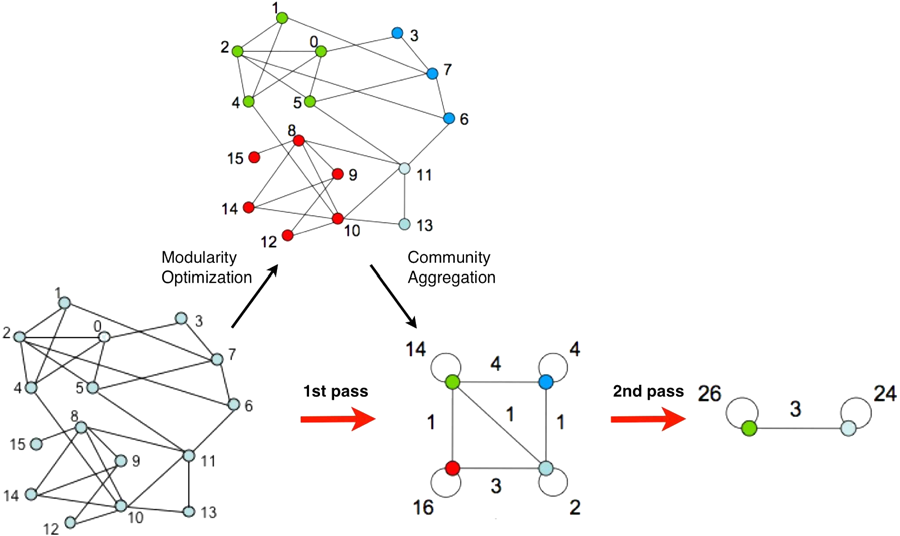
\includegraphics[width=\linewidth]{figures/blondel.png}
    \caption{An illustration of the Louvain graph clustering method. Source: \cite{lambiotte-louvain-clustering}.}
  \end{figure}

  Louvain is very effective, in part because a change (improvement) in modularity obtained by reassigning an \textbf{isolated} (not yet clustered) vertex $v_i$ to a community $C_j$ may be explicitly obtained by
  \begin{equation}
    \Delta Q=\left[ \frac{\Sigma_{in}^{(j)} + k_{i,in}^{(j)}}{2 m} - \left(\frac{\Sigma_{tot}^{(j)} + k_{i}}{2m}\right)^2 \right] - \left[ \frac{\Sigma_{in}^{(j)}}{2m} - \left(\frac{\Sigma_{tot}^{(j)}}{2m}\right)^2 - \left(\frac{k_i}{2m}\right)^2 \right] \,,
    \label{eq:blondel-deltaQ}
  \end{equation}
  (as given in the original paper) which is highly useful from a computational perspective \parencite{lambiotte-louvain-clustering}.
  Here, we have $d_{i,in}^{(j)} := \left|\left\{(v_x, v_y) \in (C_j \times C_j) \cap E \;\big|\; v_x = v_i\right\}\right|$ the number of in-cluster edges connected to vertex $v_i$ and the corresponding $\Sigma_{in}^{(j)} := \sum_{v_i \in C_j} d_{i,in}^{(j)} = \left|(C_j \times C_j) \cap E\right|$ represents the total number of edges between vertices within the same cluster $C_j$ (so neglecting edges to vertices outside $C_j$).
  Likewise, $\Sigma_{tot}^{(j)} := \sum_{v_i \in C_j} d_i$ denotes the sum of vertex degrees within the cluster $C_j$ (so including contributions to outside nodes).

  In our case, the above weightings $k_j \in \R^+$ reduce to the degrees $d_j$ alone given that we operate on an unweighted, undirected graph $G = (V, E)$. Note that the above \Cref{eq:blondel-deltaQ} simplifies to
  \begin{equation}
    \Delta Q = \cancel{\frac{\Sigma_{in}^{(j)}}{2m}} + \frac{d_{i, in}^{(j)}}{2m} - \frac{\cancel{\left(\Sigma_{tot}^{(j)}\right)^2} + 2 \Sigma_{tot}^{(j)} d_i + \cancel{d_i^2}}{4m^2} - \cancel{\frac{\Sigma_{in}^{(j)}}{2m}} + \frac{\cancel{\left(\Sigma_{tot}^{(j)}\right)^2} + \cancel{d_i^2}}{4m^2} = \frac{d_{i, in}^{(j)}}{2m} - \frac{\Sigma_{tot}^{(j)} d_i}{2m^2} \,.
    \label{eq:blondel-deltaQ-simplified}
  \end{equation}

  In more general terms, one may obtain the impact of moving a vertex $v_i \in V$ from cluster $C_a$ to $C_b$ by considering their individual contributions
  $$Q_c = \sum_{v_i \in C_c} \sum_{v_j \in C_c} \left(A_{ij} - \frac{d_i d_j}{2m}\right) = \frac{\Sigma_{in}^{(j)}}{2m} - \left(\frac{\Sigma_{tot}^{(j)}}{2m}\right)^2\,,$$
  to the total modularity $Q = \sum_{c=1}^{n_C} Q_c^{(c)}$, which are
  \begin{align*}
    \tilde{Q}_c^{(a)} & = \frac{\Sigma_{in}^{(a)} - d_{i, in}^{(a)}}{2m} - \left(\frac{\Sigma_{tot}^{(a)} - d_i}{2m}\right)^2\,, \\
    \tilde{Q}_c^{(b)} & = \frac{\Sigma_{in}^{(b)} + d_{i, in}^{(b)}}{2m} - \left(\frac{\Sigma_{tot}^{(b)} + d_i}{2m}\right)^2\,,
  \end{align*}
  after moving vertex $v_i$ from cluster $C_a$ to $C_b$.
  So the change in individual cluster modularity is given by the terms
  \begin{align*}
    \Delta Q_c^{(a)} & = \tilde{Q}_c^{(a)} - Q_c^{(a)} = \frac{-d_{i, in}^{(a)}}{2m} - \frac{d_i^2 - 2 \Sigma_{tot}^{(a)} d_i}{4m^2}\,, \\
    \Delta Q_c^{(b)} & = \tilde{Q}_c^{(b)} - Q_c^{(b)} = \frac{d_{i, in}^{(b)}}{2m} - \frac{d_i^2 + 2 \Sigma_{tot}^{(b)} d_i}{4m^2}\,,
  \end{align*}
  which yield the total modularity change $\Delta Q = \Delta Q_c^{(a)} + \Delta Q_c^{(b)}$ in the general case.
  Considering the special case when vertex $v_i \in V$ is still isolated, so when $C_a = \{v_i\}$ contains exactly that one vertex, we can further simplify to
  $$\Delta Q = \cancel{\frac{d_i^2}{4m^2}} + \frac{d_{i,in}^{(b)}}{2m} - \frac{\cancel{d_i^2} + 2 d_i \Sigma_{tot}^{(b)}}{4m^2} = \frac{d_{i,in}^{(b)}}{2m} - \frac{\Sigma_{tot}^{(b)} d_i}{2m^2} \,,$$
  because $\Sigma_{in}^{(a)} = 0$, $\Sigma_{tot}^{(a)} = d_i$ and therefore $\Delta Q_c^{(a)} = \frac{d_i^2}{4m^2}$, and we arrive at the same expression given by \cite{lambiotte-louvain-clustering} (\Cref{eq:blondel-deltaQ-simplified}), for the special case when $C_a = \{v_i\}$.
  Note that the modularity contribution $Q_c = 0$ for an empty cluster.

  This modularity gain of course is not restricted to the Louvain method in and of itself, it applies to all clustering methods and is relevant to those that operate on modularity.

  The Louvain algorithm is among the most widely used techniques for graph clustering and is available in numerous software packages.

  \subsection{Chinese Whispers}
  \label{sec:cw}
  This method, like the Louvain method, also initialises the algorithm by assigning each vertex its own category (cluster).

  \begin{algorithm}[language=pseudo, caption={\centering The \textit{Chinese Whispers} algorithm due to \cite{cw-biemann}}]
Input: an undirected graph $G = (V, E)$.
Output: a graph clustering $C = \{C_i\}_{i=1, ..., n_C}$ into $n_C$ classes.

Initialise with $n_C = n$ classes, one per vertex.
while there are changes, do
  for $v_i$ in shuffled($V$), do
    Set $s_i = \arg\max_{j} \big|\left\{(v_k, v_l) \in E \;|\; v_k = v_i \wedge v_l \in C_j\right\}\big|$.
  end
end
  \end{algorithm}

  Chinese Whispers works by iterating over all vertices in random order and reassigning them to the neighbouring category with the highest number of connected edges. If there is an equal number of edges, the reassigned cluster is chosen at random.
  This algorithm can be thought of as an agent-based simulation of a social network \parencite{cw-biemann} and is similar to Markov-Chain-Clustering \parencite{van-dongen, fortunato}.

  The algorithm may equivalently be defined by considering the \textit{class matrix} $\mathcal{D} \in \{0, 1\}^{n \times n_C}$ of a graph $G = (V, E)$ in which rows represent nodes and columns represent clusters $C_j \in C$.
  So $G_{ij} = 1$ if $v_i$ belongs to $C_j$ and $0$ otherwise.
  The algorithm operates iteratively and updates the class matrix $\mathcal{D}^{(k)}$ using
  $$M: \{0, 1\}^{n \times n_C} \mapsto \{0, 1\}^{n \times n_C}, \quad \{M(\mathcal{D})\}_{ij} = \delta_{j,\arg\max_{k\in \{0...n_C\}} \mathcal{D}_{ik}}\,,$$
  $$\mathcal{D}^{(k+1)} = M(\mathcal{D}^{(k)}) A, \quad k = 0, 1, 2, ..., N$$
  per iteration $k$, where $\mathcal{D}^{(0)} = I$ is the identity, corresponding to the initialisation of individual classes for each vertex.
  $M$ is a row-wise operation on its argument, which sets each entry in the row to zero except the (first appearing) largest one, which it sets to one.

  The paper also discusses acquisition of word classes (semantic fields), where they ran Chinese Whispers against the British National Corpus (BNC) to identify clusters of similar words.
  In order to improve performance, they cut off the 2000 most frequent words in the corpus which we will also employ later.
  This set of highly frequent words is likely to contain the \textit{core vocabulary} of the language including, but not limited to, pronouns, conjunctions, prepositions and similar parts of speech.
  \cite{cw-biemann} identified 282 clusters, 26 of which contained more than 100 words.
  Word clustering methods such as this one may even be used to improve part-of-speech tagging \parencite{ushioda-improved-pos-tagging}.

  \begin{table}[H]
    \centering
    \caption{Semantic field clusters as obtained by the Chinese Whispers algorithm applied to the British National Corpus of the English language (Source: \cite{cw-biemann}).}
    \begin{tblr}{colspec={ X[c] X[4,j,m] }}
      \hline
      Size $|C_i|$ & Sample Words                                                                            \\
      \hline
      18432        & secret, officials, transport, unemployment, farm, county, wood, procedure, grounds, ... \\
      4916         & busy, grey, tiny, thin, sufficient, attractive, vital, ...                              \\
      4192         & filled, revealed, experienced, learned, pushed, occurred, ...                           \\
      3515         & White, Green, Jones, Hill, Brown, Lee, Lewis, Young, ...                                \\
      2211         & Ian, Alan, Martin, Tony, Prince, Chris, Brian, Harry, Andrew, Christ, Steve, ...        \\
      1855         & Central, Leeds, Manchester, Australia, Yorkshire, Belfast, Glasgow, Middlesbrough, ...  \\
    \end{tblr}
  \end{table}

  A more recent work \cite{watset} describes a meta-algorithm for graph clustering in the context of Natural Language Processing, which can be based on Chinese Whispers and also other methods (hence the term 'meta').
  Their algorithm (\texttt{WATSET}) is designed for \textit{fuzzy} graph clustering which exceeds the scope of this special topic, but represents the state of the art in graph-based applications in Natural Language Processing.
  Fuzzy clustering algorithms are capable of producing \textit{soft} clusterings, which relax the requirement that all clusters are strictly disjoint (so $C_i \cap C_j = \emptyset \; \forall\,i, j$, as introduced in \Cref{def:clustering}).

  \subsubsection{Greedy Modularity}
  This modularity-optimisation based clustering method takes a very similar route as the Louvain algorithm, which is in fact based on Clauset Greedy Modularity \parencite{clauset-greedy-modularity}.
  The general idea is again based on maximizing modularity.

  \subsection{Further Approaches}
  In the following we aim to give a short overview on other available clustering methods while not going into detail.

  \subsubsection{Embeddings}
  Given a graph embedding, in which vertices are mapped to a point in $\R^n$, a frequently used measure of similarity is \textit{Cosine-Similarity}:
  $$\rho_{ij} = \arccos\left(\frac{\vec{a_i} \vec{a_j}}{\norm{\vec{a_i}}_2 \cdot \norm{\vec{a_j}}}_2\right)\,,$$
  where vectors $\vec{a_i}, \vec{a_j} \in \R^n$ denote the point corresponding to vertex $v_i, v_j$ respectively \parencite{fortunato}.
  Of course this is not quite as connected to the other methods given that it already assumes a full embedding which itself is a very involved procedure, in many instances similar to clustering methods.

  \subsubsection{Girvan-Newman}
  The clustering method deduced in \cite{girvan-newman} was a clear revolution at the time and brought graph clustering / community detection methods closer to practicians.
  It consists of multiple iterations which will each increase the number of clusters by exactly one. Each step removes the ``most valuable edge'', usually given by the edge $(v_i, v_j)$ with the highest \textit{betweenness centrality} $$b_i = \frac{2}{(n-1)(n-2)} \sum_{j=1, \neq i}^n \sum_{l=1, \neq i}^{j-1} \frac{\sigma_{jl}^{i}}{\sigma_{jl}}\,,$$ where $\sigma_{jl}$ denotes the number of shortest paths connecting vertices $v_j$ and $v_l$, and $\sigma_{jl}^i$ the number of such paths passing through vertex $v_i$ \parencite{grindrod-lecture-notes}.
  Girvan-Newman is classified as a divisive hierarchical clustering method.

  \subsubsection{Random Walks and the Map Equation}
  \label{sec:mapequation}
  This rather unusual clustering approach exploits the information-theoretic duality between community structures in networks and the length of a random walker's movements on a graph.
  The map equation describes the theoretical limit of how closely a random walk can be described by $$L(C) = q H(\mathcal{Q}) + \sum_{i=1}^{n_C} p_i H(P_i)\,,$$
  where $H(\mathcal{Q})$ and $H(P_i)$ are entropies, $p_i$ is the fraction of time the random walker spends in cluster $C_i$ and $q$ the probability that a random walker switches to another cluster at any given step \parencite{mapequation}.
  See also \Cref{fig:mapequation}, which depicts a clustering of the semantic graph $G_{12}$.

  The approach of considering random walks on a graph for the purposes of community detection is also utilised by Markov-Chain-Clustering methods.
  Simmulated Annealing for instance, where clustering transition probabilities vary over time by a ``temperature'' parameter, has proven very successful in graph clustering \parencite{fortunato}.

  \subsubsection{Spectral Clustering Methods}
  \label{sec:spectral-clustering}
  % very good resource: https://theory.epfl.ch/vishnoi/Lxb-Web.pdf
  Spectral community detection methods generally analyse the eigenvectors corresponding to the $n_C$ smallest eigenvalues and extract community information from them. A common approach is to take the rows of the eigenvector matrix as positions in space and perform k-means clustering on them, which is a spatial clustering method in $\R^n$ \parencite{fortunato}.
  For the purposes of this report, we will only consider the interesting behaviour of the eigenvalues of the graph Laplacian $L = D - A$, which can tell us how many clusters $C_i$ we may expect given the adjacency matrix $A$ and degree matrix $D$ of the graph $G = (V, E)$.
  In our case of an undirected (and connected) network, we always expect a zero eigenvalue $\lambda_1 = 0$ of the Laplacian and a number of positive eigenvalues $\lambda_i > 0$ following that. $\lambda_2$ is often referred to as the spectral gap of the graph, and its corresponding eigenvector is called the \textit{Fiedler vector} \parencite{grindrod-lecture-notes}.

  \pagebreak
  \section{Network Generation and Results}
  The text corpus and vocabulary database used for the analysis in this report is based on the database behind the \href{https://www.latin-is-simple.com/en/library/}{Latin is Simple Library} which is in the public domain. The authors of these works are Augustus, Caesar, Cato, Cicero, Ovid, Hyginus, Titus, Vergil, Seneca the younger and Seneca the elder.
  In order to avoid incorporating too many grammatical particles / utility words, according to common practice \parencite{cw-biemann}, we have removed the 2000 most frequent words from the dataset.
  As Latin is a highly inflected language, we took great care to consider inflections of a Latin word as the same vocabulary entry / vertex on the graph.

  We will consider the semantic graph built by iterating the text corpus with neighbouring radii $r = 4$, $r = 8$ and $r = 12$ and refer to the resulting graphs as $G_4$, $G_8$ and $G_{12}$ respectively.
  So words which appear at most $r$ words apart in the text will be represented by connected vertices in $G_r$.
  Note that a higher neighbouring radius $r$ naturally yields a higher number of edges.

  \begin{table}[H]
    \centering
    \caption{Clustering results for the corpus-generated semantic networks $G_4$, $G_8$ and $G_{12}$ with 10843 nodes and 1.1 million, 1.8 million and 2.4 million edges, respectively.}
    \begin{tblr}{rlcrrrr}
      \hline
      Graph & Method & $Q$ & Runtime [s] & $n_C$ & Avg. size & Max size \\
      \hline
      $G_4$ & louvain & 0.1307 & 25.091 & 9 & 1204.78 & 4066 \\
      $G_4$ & chinese-whispers & 0.0168 & 126.342 & 1929 & 5.62 & 39 \\
      $G_4$ & greedy-modularity & 0.1150 & 1993.632 & 39 & 278.03 & 4836 \\
      $G_8$ & louvain & 0.1189 & 58.373 & 5 & 2168.60 & 3748 \\
      $G_8$ & chinese-whispers & 0.0142 & 179.585 & 1625 & 6.67 & 43 \\
      $G_8$ & greedy-modularity & 0.1074 & 2211.958 & 25 & 433.72 & 5375 \\
      $G_{12}$ & louvain & 0.1150 & 43.723 & 4 & 2710.75 & 3465 \\
      $G_{12}$ & chinese-whispers & 0.0011 & 242.934 & 365 & 29.71 & 9778 \\
      $G_{12}$ & greedy-modularity & 0.1033 & 2324.660 & 12 & 903.58 & 5520
    \end{tblr}
    \label{table:timings}
  \end{table}

  \Cref{table:timings} shows the individual runtimes of each algorithm on graphs $G_4$, $G_8$ and $G_{12}$, along with the resulting modularity $Q$ of a clustering into $n_C$ clusters with average and maximum size given in the table as well.
  For graphs of this size, Girvan-Newman did not converge within a day, not even for the first iteration which would have only yielded a bipartition of the graph.
  From \Cref{table:timings}, one can clearly see that the Louvain method is not only the fastest but also yields the highest modularity $Q$, which is perhaps unsurprising given that it is based on optimisation of $Q$.
  However, it yields a very small number of very heterogeneously sized clusters which is not necessarily ideal for the application of semantic field analysis.

  Followed closely after it, we have the Greedy Modularity method which also yields a fairly high modularity (slightly higher than 0.1), but has runtime of about half an hour, which is much longer than the runtime of Louvain which is on the order of seconds.
  This comparison may put the fantastic performance improvement of the Louvain method into perspective, given that it is based on the Greedy Modularity method.

  The runner-up in terms of runtime is the Chinese Whispers algorithm which takes only a few minutes, but yields a very poor modularity $Q$.
  However, Chinese Whispers returns the most usable semantic fields which are of average size 6 for $G_4$ and $G_8$ and comprise around 30 words for $G_{12}$. Samples of the resulting semantic fields may be found in \Cref{table:samples}.
  Similar results are found for the small clusters obtained by the modularity optimisation methods (Louvain and Greedy Modularity), but words contained in larger clusters ($> 1000$ vertices) only appear connected in a grammatical sense, so only loosely connected by the literature context or even word type.

  \begin{table}[H]
    \centering
    \caption{Clustering results for Zachary's Karate Club Graph \parencite{karate-club}.}
    \begin{tblr}{lcrrrr}
      \hline
      Method & $Q$ & Runtime [s] & $n_C$ & Avg. size & Max size \\
      \hline
      greedy-modularity & 0.4110 & 0.006 & 3 & 11.33 & 17 \\
      girvan-newman & 0.3477 & 0.145 & 2 & 17.00 & 19 \\
      louvain & 0.4439 & 0.002 & 4 & 8.50 & 14 \\
      chinese-whispers & 0.3920 & 0.004 & 7 & 4.86 & 11
    \end{tblr}
    \label{table:karate}
  \end{table}

  For reference, we also applied each algorithm to the standard Zachary's Karate Club graph with runtimes, modularities and cluster sizes available in \Cref{table:karate}.
  The interested reader may find further runtime analysis tables and computational complexities in \cite{watset} as well as \cite{fortunato}.

  \begin{table}
    \centering
    \caption{Some resulting clusters (semantic fields) in $G_4$, the network of words whose edges correspond to distances of at most 4 words from one another in the Latin text corpus, extracted using the Chinese Whispers clustering method.}
    \begin{tblr}{colspec={ X[c] X[4,j,m] }}
      \hline
      Size $|C_i|$ & Sample Words                                                                            \\
      \hline
      4 & conterritus (frightened), minitabundus (threatening), infensus (hostile), properus (quick) \\
      6 & hibernus (wintry), tardus (slow), upilio (shepherd), formosus (beautiful), hibernum (winter camp (pl.)), subulcus (swineherd) \\
      4 & fraus (deceit), fraus (fraud), infitiatio (denial), furtum (theft) \\
      6 & fraxinus (ash-tree), laurea (laurel/bay tree), fraxinus (of ash), corylus (hazel-tree), edurus (very hard), abies (fir tree/wood) \\
      4 & vicina (neighbor), vicinus (nearby), vicinus (neighbor), vicinum (neighborhood) \\
      7 & repens (sudden), susurro (whisperer), nutrix (nurse), susurrus (whispering), immanitas (brutality), susurrus (whisper), diritas (frightfulness) \\
      8 & Aegyptius (Egyptian), Aethiopia (Ethiopia), siccitas (dryness), Aegyptus (Egypt), desertum (desert), Aegyptius (Egyptian), aspis (asp), Arabia (Arabia) \\
      8 & Marius (Marius), Maria (Mary), caelia (kind of beer), citrum (wood of citron tree), alternatus (alternate), citrus (African citrus tree), series (row), citrus (lemon tree) \\
      6 & inexspectatus (invincible), armum (arms (pl.)), tribunicius (of/belonging to tribune), intutus (defenseless), Arma (Arms), arma (weapons) \\
      2 & globosus (round), rotundus (round)
    \end{tblr}
    \label{table:samples}
  \end{table}

  \begin{figure}
    \centering
    \begin{subfigure}[b]{0.3\textwidth}
      \centering
      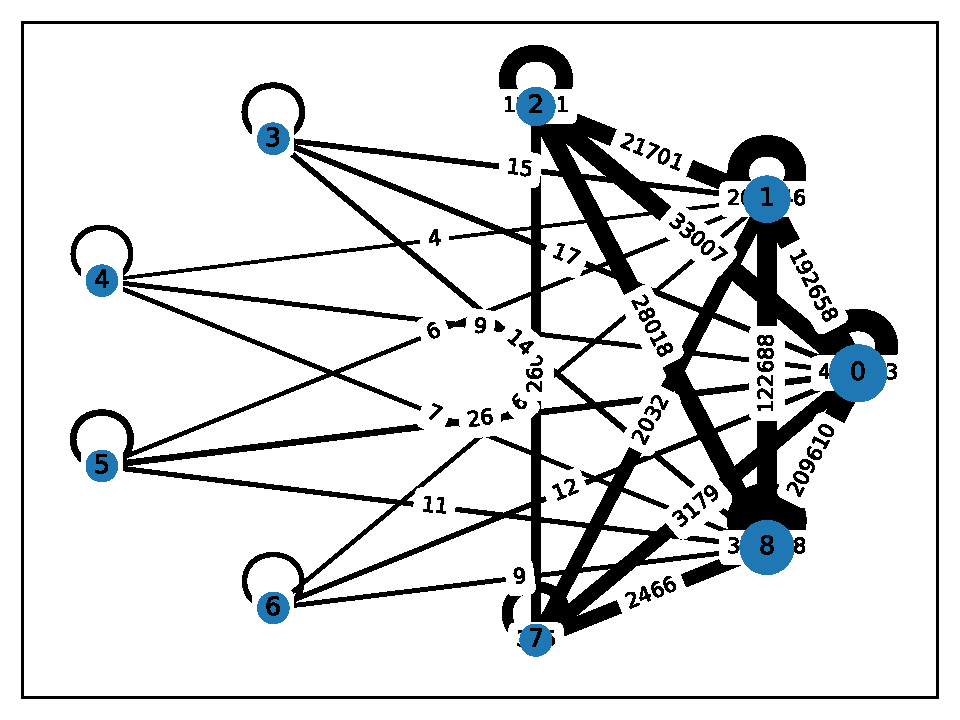
\includegraphics[width=\textwidth]{figures/H-4-louvain.pdf}
      \caption{Clusters of $G_4$.}
      \label{fig:h-4}
    \end{subfigure}
    \hfill
    \begin{subfigure}[b]{0.3\textwidth}
      \centering
      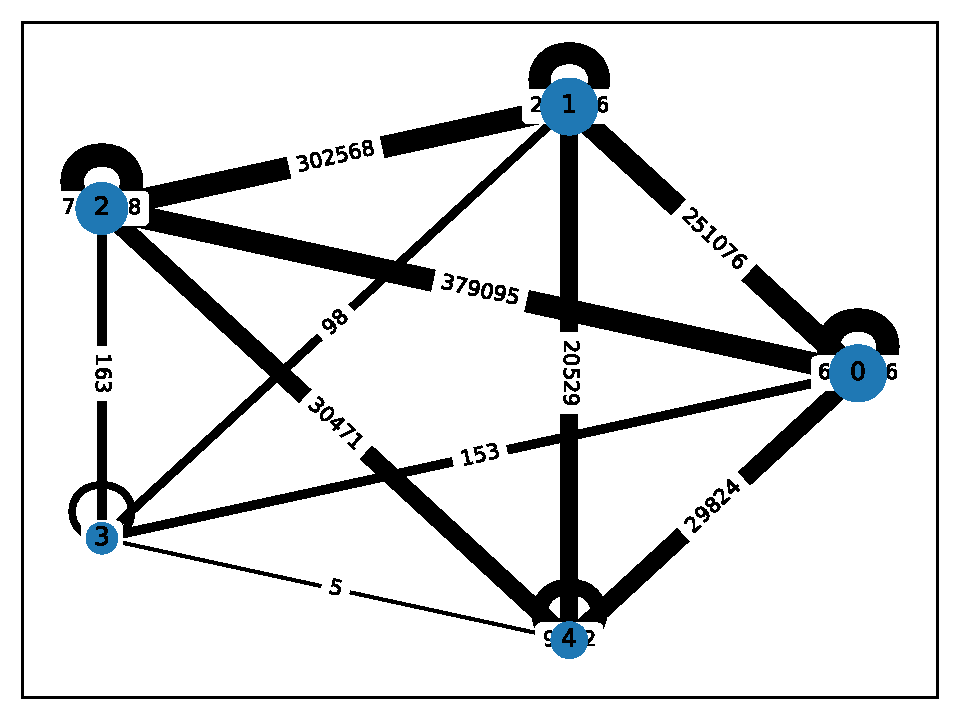
\includegraphics[width=\textwidth]{figures/H-8-louvain.pdf}
      \caption{Clusters of $G_8$.}
      \label{fig:h-8}
    \end{subfigure}
    \hfill
    \begin{subfigure}[b]{0.3\textwidth}
      \centering
      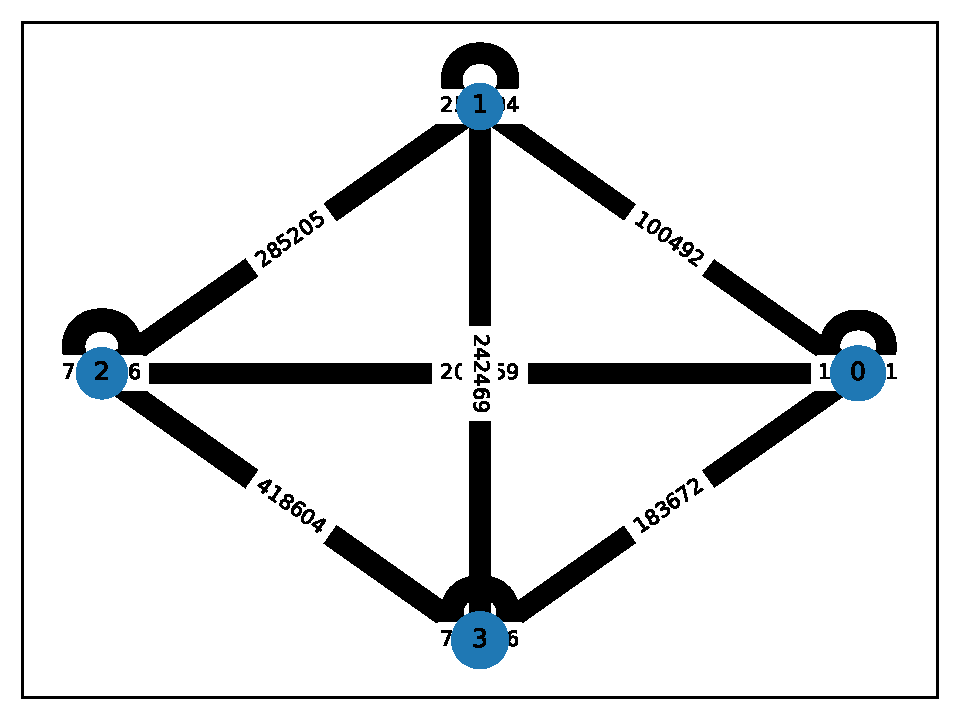
\includegraphics[width=\textwidth]{figures/H-12-louvain.pdf}
      \caption{Clusters of $G_{12}$.}
      \label{fig:h-12}
    \end{subfigure}
    \caption{The weighted graphs of clusters and their number of inter-cluster edges connecting them for $G_4$, $G_8$ and $G_{12}$, as obtained by the Louvain method. The graphs shown also contain edges from vertices (representing clusters) back to themselves (i.e. diagonal entries in the adjacency matrix) which represent the number of edges within the corresponding cluster.}
    \label{fig:three graphs}
  \end{figure}

  The clusters obtained by the Louvain method are depicted in \Cref{fig:three graphs}, using a similar visualisation method as InfoMap \Cref{fig:mapequation}.
  The semantic connectedness of the Louvain clusters is not immediately apparent due to the large size of the clusters.

  \begin{figure}[H]
    \centering
    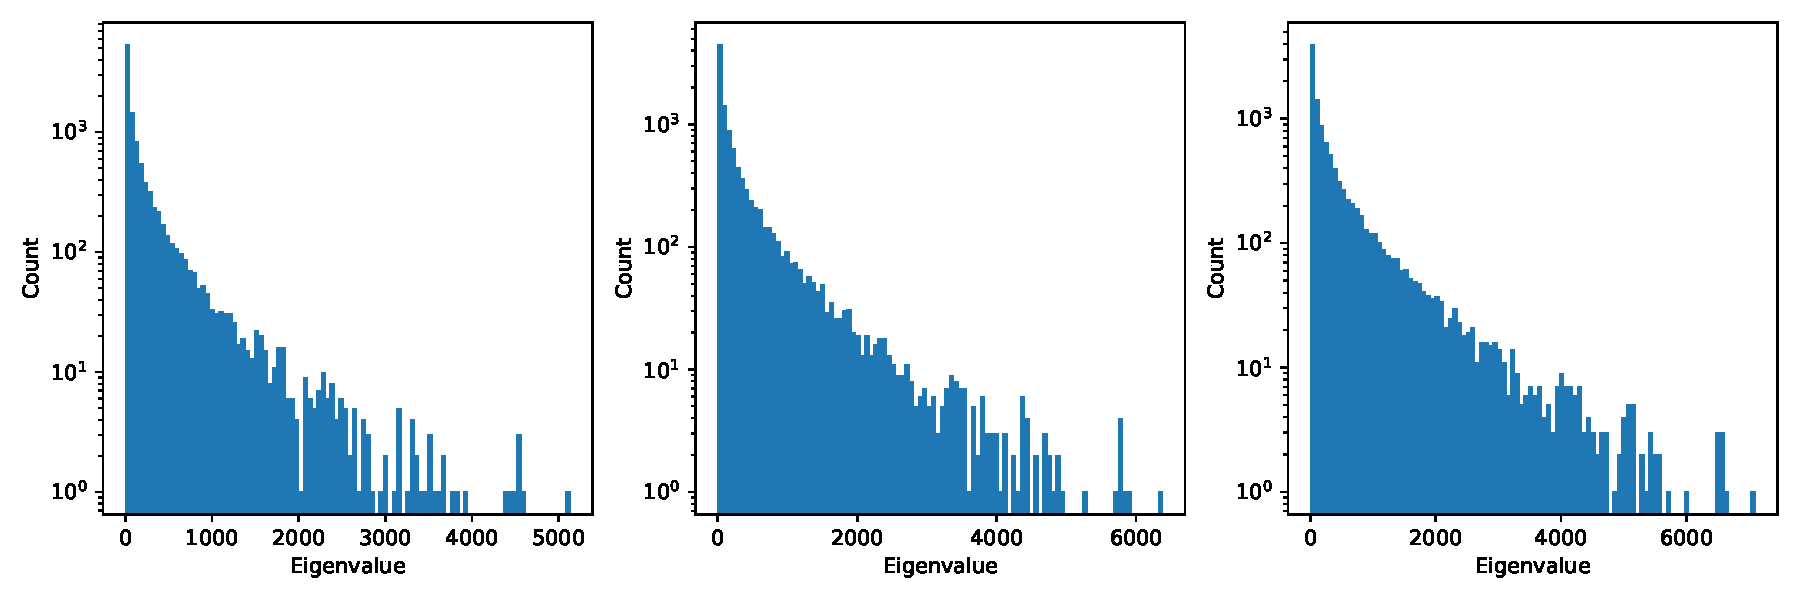
\includegraphics[width=\linewidth]{figures/spectrum-of-laplacian.pdf}
    \caption{From left to right: Histograms of the eigenvalue spectrum of the graph Laplacians $L = D - A$ of $G_4$, $G_8$ and $G_{12}$, respectively.}
    \label{fig:laplacians}
  \end{figure}

  \Cref{fig:laplacians} depicts a histogram of the spectra of the graph Laplacians $L$ for the given three graphs.
  From here, one can make conclusions about the expected number of clusters in the network. $G_4$, for instance, has a clear gap of eigenvalues around $\lambda = 2000$, which suggests a partitioning into about 2000 clusters of $G_4$. Chinese Whispers, a probabilistic algorithm, yields almost exactly that number (within a \SI{1}{\percent} error tolerance!).
  A similar argument can be made for both modularity-optimisation methods upon closer inspection of the spectrum, although by far not as clearly.
  The graphs $G_8$ and $G_{12}$ are far more connected than $G_4$ and therefore yield a lower number of clusters.
  Which is expected, but not very easily visible in the eigenvalue spectrum.

  \pagebreak
  \section{Conclusion}
  In this report, we have introduced a few basic notions of network theory, discussed in detail two graph clustering approaches, the Louvain method (cf. \Cref{sec:louvain}), where we rederived the gain in modularity upon clustering of an isolated vertex, and Chinese Whispers (cf. \Cref{sec:cw}).
  These methods make significant progress in a problem that is usually NP-hard.
  Using a neighbourhood-based approach with parameter $r$, we constructed large networks $G_4$, $G_8$ and $G_{12}$ from an original classicist Latin literature corpus and applied the abovementioned methods to cluster them.
  The constructed graphs' vertices only represent principal words, so the text corpus was analyzed up to grammatical equivalences in the Latin language which is entirely original.

  We then analyzed three clustering methods from a computational perspective with results presented in \Cref{table:timings}, \Cref{table:samples} and visualised in \Cref{fig:three graphs}.
  The Louvain method was by far the fastest algorithm for our application.
  The eigengap of the spectrum of the Laplacian then yielded a good estimate for the expected number of clusters.

  As the author describes in \cite{cw-biemann}, Chinese Whispers generally produces a fairly high number of clusters as compared to other methods, which one may circumvent by adjusting either the convergence condition or introduce a minimum cluster size through minor adjustments of the algorithm.
  Similar measures may be taken for the other algorithms.
  In our case however, the clusters produced make a reasonable impression when looking at the words contained therein.

  Even better results for the semantic fields could be achieved by incorporating an even larger text corpus to prevent clustering of words which are only used once or twice, so only in the context given by the literature.

  \pagebreak
  \printbibliography
\end{document}
